\documentclass[t,% Place text of slides at the (vertical) top of the slides
brazilian,% Brazilian Portuguese, FTW!
11pt,% Standard font size
aspectratio=169,% Aspect ratio 16:9 (widescreen)
table% xcolor option
]{beamer}

\setbeamercolor{footnote mark}{fg=red}

\usetheme{Boadilla}
\setbeamertemplate{navigation symbols}{}
\setbeamertemplate{frametitle continuation}{}
\setbeamertemplate{page number in head/foot}[framenumber]
\setbeamertemplate{enumerate items}[default]
\setbeamertemplate{itemize items}[circle]
\setbeamercovered{transparent}
\setbeamerfont{frametitle}{size=\normalsize}

\usepackage{babel}
\usepackage[utf8]{inputenc}
\usepackage[T1]{fontenc}
\usepackage{lmodern}

\usepackage{graphicx}
\setkeys{Gin}{keepaspectratio}

\usepackage{amssymb,amsfonts,amsmath}
\usepackage{mathtools}

\usepackage{siunitx}
\sisetup{locale = FR}

\usepackage{tikz}
\usetikzlibrary{calc}

\usepackage{pgffor}
\usepackage{etoolbox}

% \usepackage{colortbl}

\usepackage{tcolorbox}

\usepackage{pgfplots}
\pgfplotsset{compat=1.18}

\newcommand{\esima}{\textordfeminine }
\newcommand{\esimo}{\textordmasculine }

\newcommand{\vboxcorr}[2]{%
    \resizebox{!}{\totalheight-#1}{#2}%
}
\newcommand{\hboxcorr}[2]{%
    \resizebox{\width-#1}{!}{#2}%
}

\DeclareMathOperator{\arctg}{arctg}
\DeclareMathOperator{\sen}{sen}
\DeclareMathOperator{\arcsen}{arc sen}

\def\Disciplina{Fenômenos de Transporte}
\def\Professor{Rodrigo de Farias Gomes}
\def\Periodo{Período 2025.1}

\title{\Disciplina}
\author{\Professor}
\date{\Periodo}

\begin{document}

\begin{frame}
    \titlepage
\end{frame}

\begin{frame}{Informações gerais}
    \begin{itemize}
        \item Nome: {\fontfamily{augie}\selectfont Rodrigo de Farias Gomes}
        \item Telefone (somente mensagens): (92) 9 9405-1724
        \item E-mail: shpnft@gmail.com
        \item Sala: 201b, Bloco E (2\esimo{} pavimento)
    \end{itemize}
\end{frame}

\begin{frame}{Avaliação}
    \begin{itemize}
        \item A avaliação será na forma de 3 notas: \(N_1\), \(N_2\) e \(N_3\)
        \item A média dos exercícios escolares (\(ME\)) será dada por
            \[
                ME=\frac{N_1+N_2+N_3}{3}
            \]
        \item Se \(MEE \geq 8,0\), então a média final (\(MF\)) será igual à \(MEE\)
        \item Se \(MEE < 8,0\), então
            \[
                MF=\frac{2\times MEE+PF}{3}
            \]
            onde PF é a nota da \textbf{prova final}
        \item A prova final abordará o mesmo \textit{conteúdo} da última prova realizada
        \item Se \(MF \geq 5,0\) e a frequência em sala for maior que 75\%, o aluno está aprovado
    \end{itemize}
\end{frame}


\begin{frame}<1>[label=ementa]{Ementa de \Disciplina}
    \begin{itemize}
        \item Conceitos e definições fundamentais
        \item Conceitos de Fenômenos de Transporte e
            Analogia entre os Processos Difusivos Unidimensionais de
            Transferência de Movimento Linear, de Calor e de Massa
        \item Fundamentos da Estática dos Fluidos
        \item Descrição e Classificação de Escoamentos
        \item Introdução à Análise de Escoamentos na Formulação de Volume de Controle
        \item Introdução à Análise Diferencial de Escoamentos
        \item Introdução à Transferência de Calor
        \item Introdução à Condução Unidimensional de Calor em Regime Permanente
        \item Introdução à Condução de Calor em Regime Transiente
        \item Introdução à Transferência de Massa
    \end{itemize}
\end{frame}

\begin{frame}{Livro}
    \centering
    \vboxcorr{27pt}{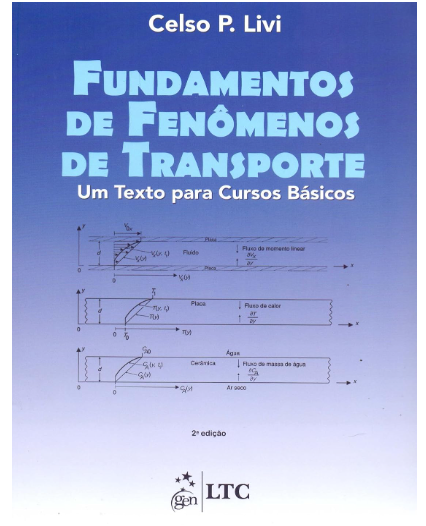
\includegraphics[height=\textheight]{images/Captura de tela de 2025-03-18 15-21-27.png}}
\end{frame}

\begin{frame}{Capítulos do Livro}
    \centering
    \vboxcorr{27pt}{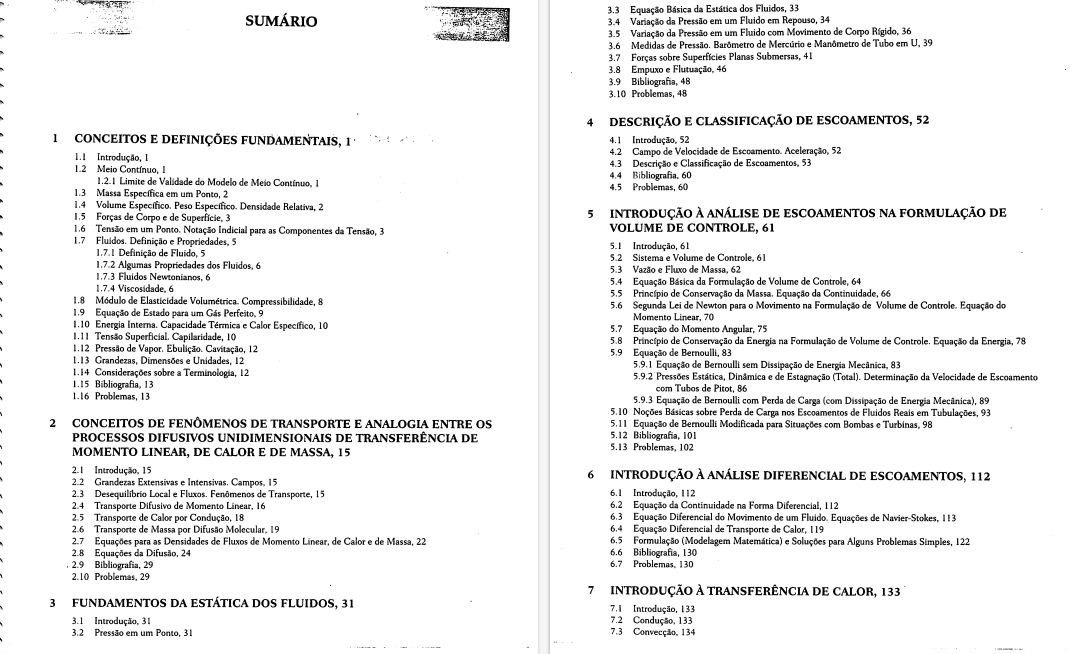
\includegraphics[height=\textheight]{images/Captura de tela de 2025-03-18 15-25-51.png}}
\end{frame}

\begin{frame}{Capítulos do Livro}
    \vboxcorr{27pt}{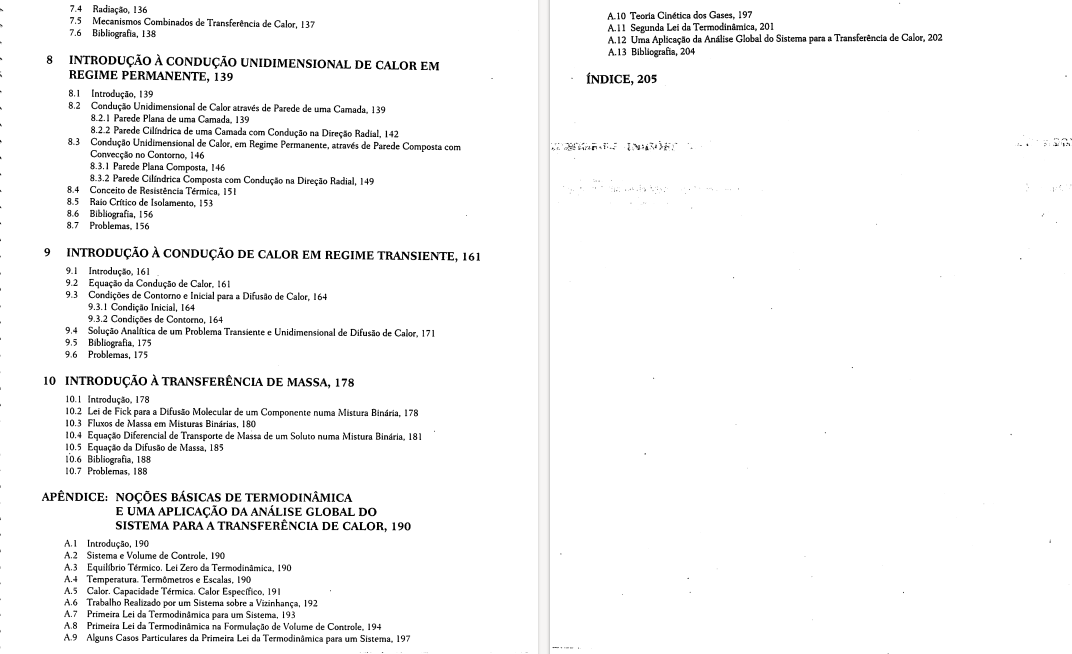
\includegraphics[height=\textheight]{images/Captura de tela de 2025-03-18 15-26-08.png}}
\end{frame}

\begin{frame}{Massa específica, volume específico e peso específico}
    \begin{itemize}
        \item Massa específica
            \[
                \rho = \lim_{\Delta V \to \delta V} \frac{\Delta m}{\Delta V} 
            \]
            onde:
            \begin{description}
                \item[\(\Delta m\)] é a massa contida no volume \(\Delta V\)
                \item[\(\delta V\)] é o menor volume onde seja válido o \textbf{modelo contínuo}
            \end{description}
        \item Volume específico
            \[
                v=\frac{1}{\rho}
            \]
        \item Peso específico
            \[
                \gamma = \rho g
            \]
    \end{itemize}
\end{frame}

\begin{frame}{Forças}
    \begin{itemize}
        \item Forças de corpo são aquelas que se manifestam através da interação com um campo e 
            atuam sem a necessidade de um contato entre as superfícies dos corpos.

            Exemplos: força peso, força elétrica, força magnética

            Forças de corpo são proporcionais ao volume dos corpos\footnote{Somente no caso de corpos uniformes}

        \item Forças de superfície são aquelas que atuam sobre um sistema através de contato com a fronteira do mesmo

            Exemplos: força de atrito, forças devido à \textit{pressão}

            Forças de superfície são proporcionais à área da superfície sobre a qual atuam
            \footnote{Somente no caso de corpos com superfícies uniformes}
    \end{itemize}
\end{frame}

\begin{frame}{Tensão e pressão}
    \begin{itemize}
        \item  A tensão é definida como a força por unidade de área aplicada a
            um corpo. Mas vimos em Física Geral II que pressão também é força
            por unidade de área. Qual a diferença?
        \item Pressão é uma grandeza \textbf{escalar} que só considera a componente \textit{normal} da força aplicada na superfície,
            enquanto a tensão é uma grandeza \textbf{tensorial} que considera todas as componentes
            \[
                \vec{\vec{T}}=
                \begin{bmatrix}
                    \sigma_{xx} & \tau_{xy} & \tau_{xz} \\ 
                    \tau_{yx} & \sigma_{yy} & \tau_{yz} \\
                    \tau_{zx} & \tau_{zy} & \sigma_{zz}
                \end{bmatrix}
            \]
            onde as \textbf{tensões normais} \(\sigma_{ii}\) são definidas como
            \[
                \sigma_{ii} = \lim_{\Delta A_i \to 0} \frac{\Delta F_i}{\Delta A_i}
            \]
            e as \textbf{tensões cisalhantes} (tangenciais) \(\tau_{ij}\) são definidas como
            \[
                \tau_{ij} = \lim_{\Delta A_i \to 0} \frac{\Delta F_j}{\Delta A_i}
            \]
    \end{itemize}
\end{frame}

\begin{frame}{Fluidos}
    \begin{itemize}
        \item A definição mais elementar de fluido diz: ''Fluido é uma
            substância que não tem uma forma própria, assume o formato do
            recipiente''
        \item Se o problema fundamental fosse apenas reconhecer os fluidos, a
            definição apresentada seria perfeitamente suficiente para essa
            finalidade
        \item Entretanto, vamos montar uma definição baseada na tensão de
            cisalhamento aplicada
        \item Seja um sólido preso entre duas placas planas
            \begin{center}
                \hboxcorr{22pt}{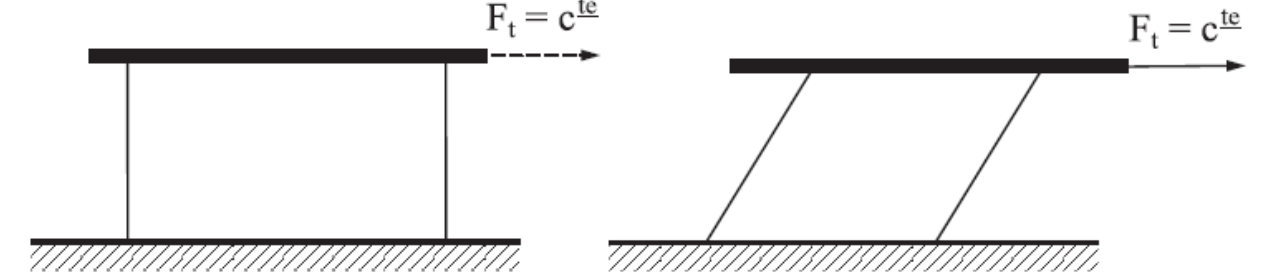
\includegraphics[width=\textwidth]{images/Captura de tela de 2025-03-25 15-37-33.png}}
            \end{center}
        \item Nota-se que o sólido se deforma até alcançar uma posição de
            equilíbrio estático
    \end{itemize}
\end{frame}

\begin{frame}
    \begin{itemize}
        \item Agora vamos colocando-se um fluido entre as placas, ''assumindo''
            que seja possível visualizar um certo volume \(ABCD\) do fluido
            \begin{center}
                \hboxcorr{22pt}{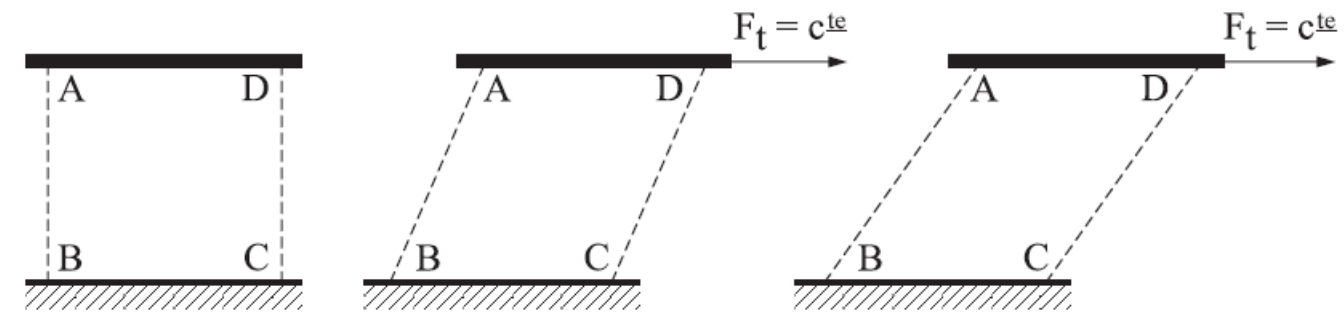
\includegraphics[width=\textwidth]{images/Captura de tela de 2025-03-25 15-42-52.png}}
            \end{center}
        \item \textbf{Princípio da Aderência}: Os pontos de um fluido, em
            contato com uma superfície sólida, aderem aos pontos dela, com os
            quais estão em contato
        \item Ou seja,a velocidade do fluido em contato com a placa será a igual
            a velocidade da placa
        \item Ou seja, os fluidos se deformam continuamente
    \end{itemize}
\end{frame}

\begin{frame}
    \begin{itemize}
        \item Ou seja, ''Fluido é uma substância que se deforma continuamente sob a ação
            de uma tensão de cisalhamento, \textbf{por menor que ela seja}''
        \item Existindo tensão cisalhante o fluido entra em movimento, ou seja, ocorre \textbf{escoamento}
        \item Os fluidos se moldam ao formato dos recipientes que os contêm \footnote{Por quê?}
        \item Um fluido é incompressível se, ao ser submetido a uma tensão normal, não há
            variação volumétrica
        \item Para um fluido em repouso, a tensão é exclusivamente normal, sendo seu valor
            chamado de pressão estática \(p\) que, em um ponto, é igual em qualquer direção, ou seja
            \[
                \sigma_{xx}=
                \sigma_{yy}=
                \sigma_{zz}=-p
            \]
    \end{itemize}
    \pause
    \begin{block}{Problema 1.1 do livro texto}
        Os líquidos e gases são fluidos, mas apresentam características diferentes. Descreva as propriedades
        que diferenciam os gases dos líquidos
    \end{block}
\end{frame}

\begin{frame}{Viscosidade}
    \begin{itemize}
        \item Vamos analisar um pouco mais o caso do fluido entre placas
            \begin{center}
                \hboxcorr{22pt}{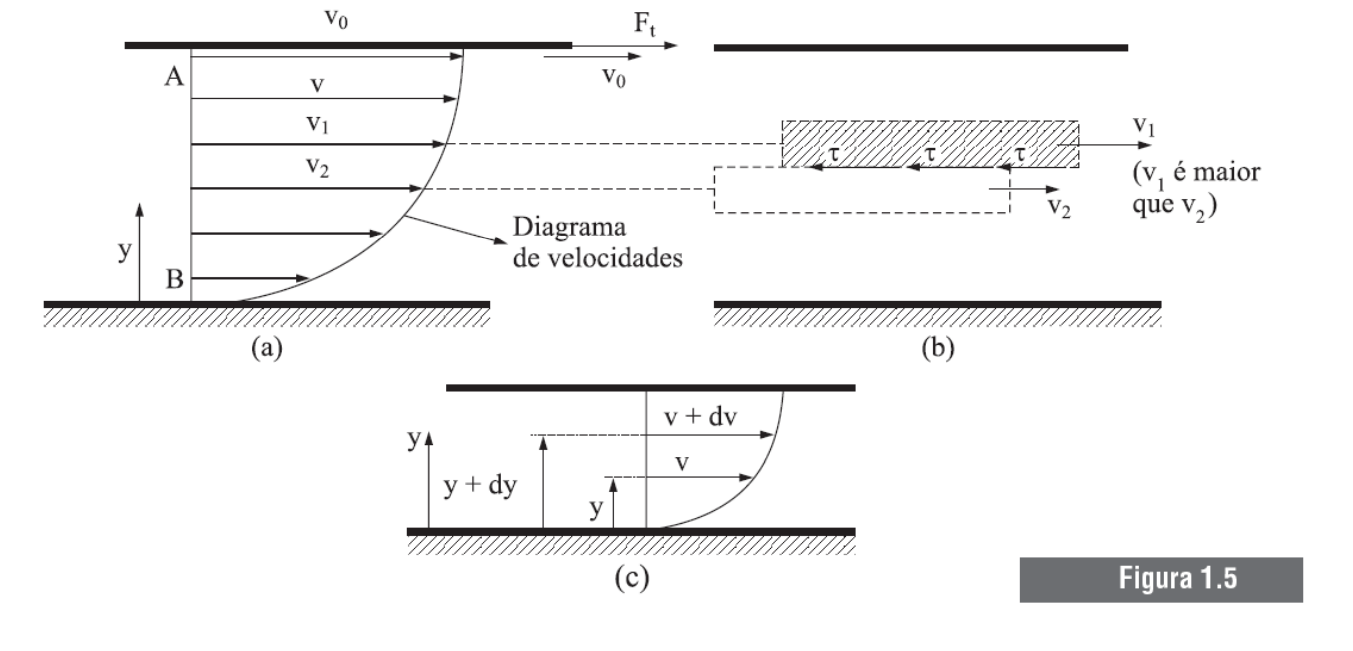
\includegraphics[width=\textwidth]{images/Captura de tela de 2025-03-25 16-11-12.png}}
            \end{center}
    \end{itemize}
\end{frame}

\begin{frame}
    \begin{itemize}
        \item Note que a diferença de velocidade \(v_1-v_2\) entre duas ''camadas'' do fluido pode ser
            explicada pela tensão de cisalhamento \(\tau\)
        \item Newton descobriu que em muitos fluidos \(\tau\) é proporcional a variação da velocidade com \(y\)
            \[
                \tau = \mu \frac{dv}{dy}
            \]
        \item Essa equação\footnote{No livro há um sinal negativo, mas vou
            omiti-lo por enquanto} é conhecida como \textbf{Lei de Newton para
            a Viscosidade} e \(\mu\) é a \textbf{viscosidade absoluta ou dinâmica}
        \item Os fluidos que obedecem a essa lei são ditos \textbf{fluidos newtonianos}, enquanto que
            os outros são chamados de \textbf{não newtonianos}
        \item Aqui só vamos tratar de fluidos newtonianos
    \end{itemize}
\end{frame}

\begin{frame}
    \begin{itemize}
        \item Podemos dizer que ''viscosidade é a propriedade que indica a maior ou menor dificuldade
            do fluido escoar''
        \item A viscosidade é causada fundamentalmente pela coesão intermolecular 
            e pela \textit{transferência de momento linear} através do fluido
        \item A viscosidade depende da temperatura, sendo que ela aumenta com a temperatura nos 
            gases e diminui com a temperatura nos líquidos\footnote{No livro texto há uma explicação para isso na página 8}
        \item No SI, a unidade da viscosidade absoluta é \(\si{Pa\cdot s}\)
        \item A viscosidade cinemática do fluido é dada por
            \[
                \nu = \frac{\mu}{\rho}
            \]
            onde \(\rho\) é a massa específica do fluido. A unidade de \(\nu\) no SI é 
            \(\si{m^2/s}\)
    \end{itemize}
\end{frame}

\begin{frame}{Problemas}
    \begin{itemize}
        \item [1.3] A figura 1.7 mostra o esquema de um escoamento de água entre duas placas
            planas horizontais de grandes dimensões e separadas por uma distância \(d\) pequena.
            A placa inferior permanece em repouso, enquanto a placa superior está em movimento com 
            velocidade \(V_x\) constante, de forma que resulta uma distribuição linear de velocidade
            de escoamento de água. Sendo a viscosidade da água \(\mu=\SI{1e-3}{Pa\cdot s}\), determine
            \begin{enumerate}[a)]
                \item o gradiente de velocidade de escoamento
                \item a tensão de cisalhamento na placa superior
            \end{enumerate}
    \end{itemize}
    \centering
    \vboxcorr{115pt}{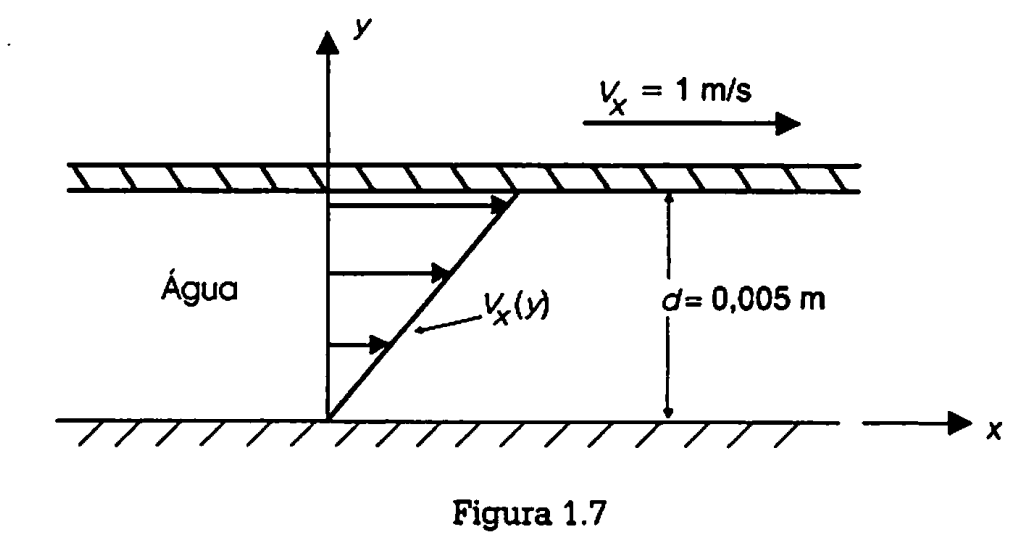
\includegraphics[height=\textheight]{images/Captura de tela de 2025-03-25 16-57-30.png}}
\end{frame}

\begin{frame}
    \begin{itemize}
        \item [1.5] A figura 1.8 mostra um esquema de distribuição de
            velocidade para um escoamento laminar de um fluido newtoniano,
            totalmente desenvolvido \footnote{Escoamento totalmente
            desenvolvido é aquele onde o perfil de velocidade não varia ao
            longo do eixo do tubo}, num duto de seção circular de diâmetro
            constante, dada por
            \[
                V_z(r) = V_\text{máx}\left[1-\left(\frac{r}{R}\right)^2\right]
            \]
            onde \(V_\text{máx}\) é a velocidade máxima do perfil (distribuição), que ocorre
            no centro da seção, e \(R\) é o raio interno do duto

            Sendo \(\mu\) a viscosidade dinâmica do fluido, determine 
            \begin{enumerate}[a)]
                \item a distribuição de tensões de cisalhamento \(\tau_{rz}\) no escoamento
                \item a força por unidade de comprimento que o escoamento exerce sobre a parede 
                    do duto
            \end{enumerate}
    \end{itemize}
    \centering
    \vboxcorr{161pt}{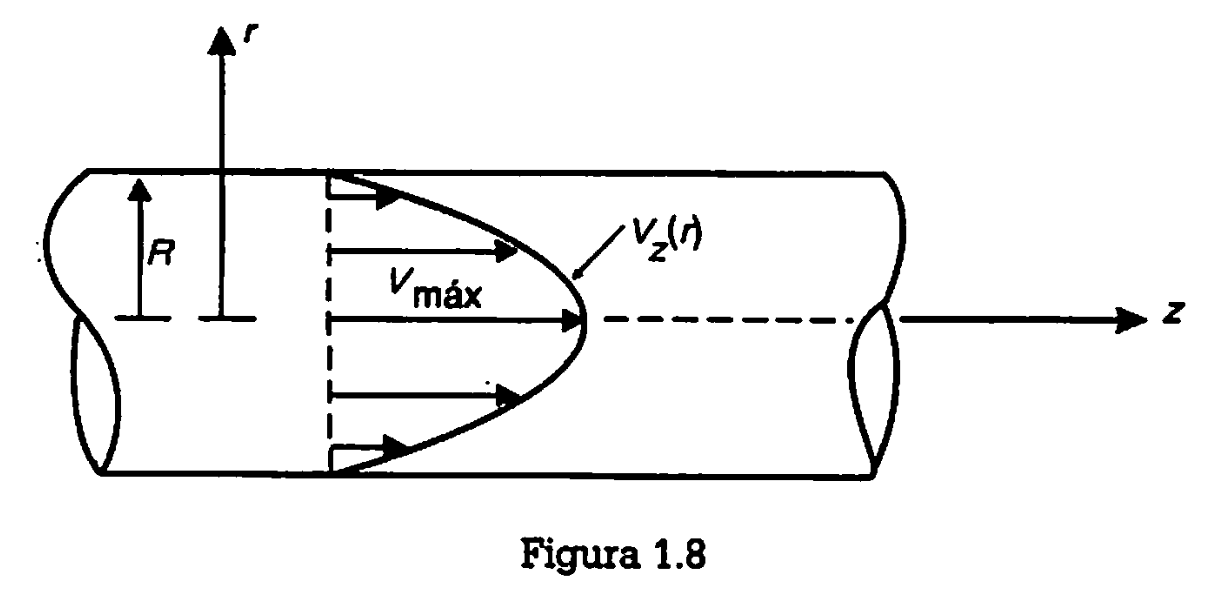
\includegraphics[height=\textheight]{images/Captura de tela de 2025-03-25 17-07-55.png}}
\end{frame}

\begin{frame}
    \begin{itemize}
        \item[1.6] A figura 1.9 mostra um esquema de um escoamento laminar, totalmente desenvolvido e em
            regime permanente, de um fluido newtoniano, entre duas placas paralelas e estacionárias, de 
            grandes dimensões e separadas de uma distância \(h\) pequena. A distribuição de velocidade
            de escoamento é dada por
            \[
                V_x (y) = V_\text{máx} \left[ 1-\left(\frac{2y}{h}\right)^2\right]
            \]

            Determine a força cisalhante, por unidade de área, exercida pelo escoamento sobre a placa superior.
    \end{itemize}
    \centering
    \vboxcorr{130pt}{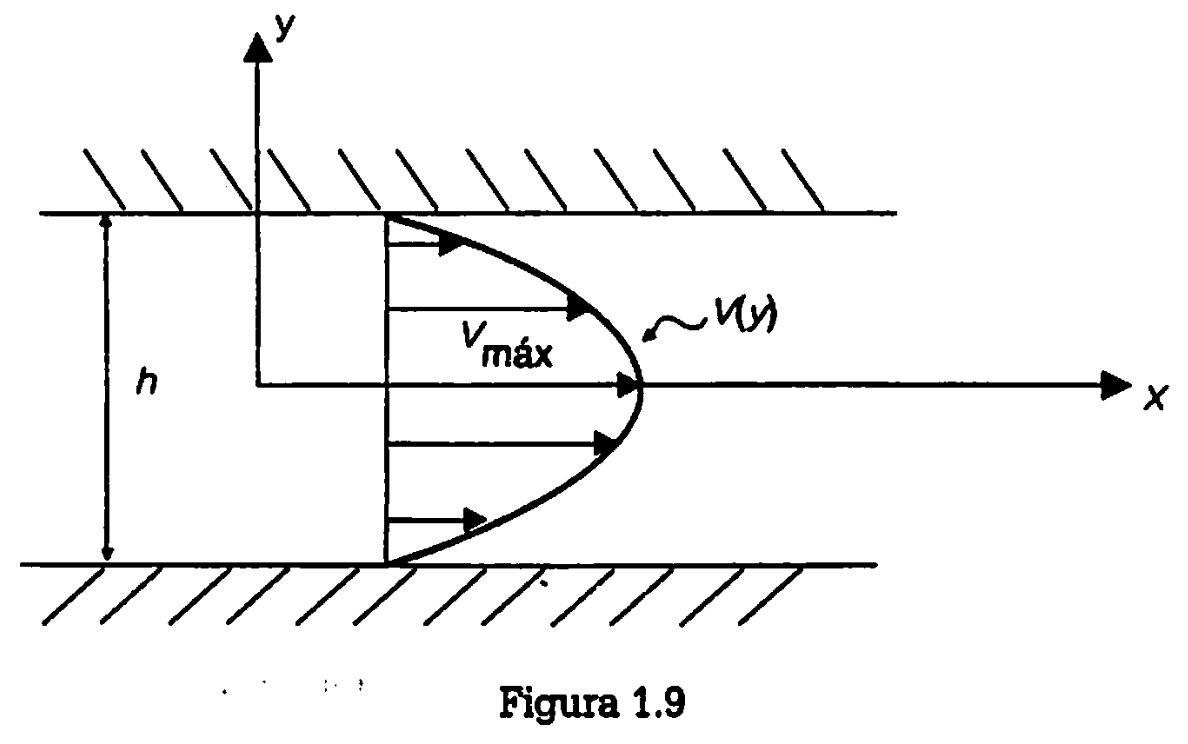
\includegraphics[height=\textheight]{images/Captura de tela de 2025-03-25 17-20-53.png}}
\end{frame}

\begin{frame}{Atividade 1}
    \begin{itemize}
        \item Vale 10\% da \(N_1\)
        \item Individual
        \item Leia as seções 1.8 e 1.9 do livro texto
        \item Resolva os problemas 1.7, 1.8, 1.9 e 1.10
        \item Data de entrega: 11/04/2025
        \item Google Sala de Aula: 
            https://classroom.google.com/c/NzYyNDc5OTQ1OTUx?cjc=\textcolor{blue}{mvcaim6v}
    \end{itemize}
\end{frame}

\begin{frame}[c]{Algumas unidades \textit{diferentes}}
    \begin{columns}
        \begin{column}{0.45\textwidth}
            \centering
            Viscosidade dinâmica
            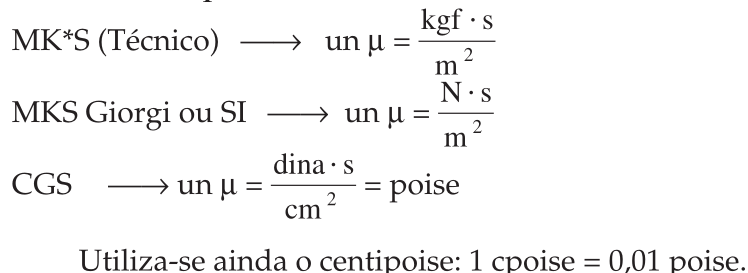
\includegraphics[width=\textwidth]{images/Captura de tela de 2025-03-26 16-53-52.png}
        \end{column}

        \begin{column}{0.45\textwidth}
            \centering
            Viscosidade cinemática
            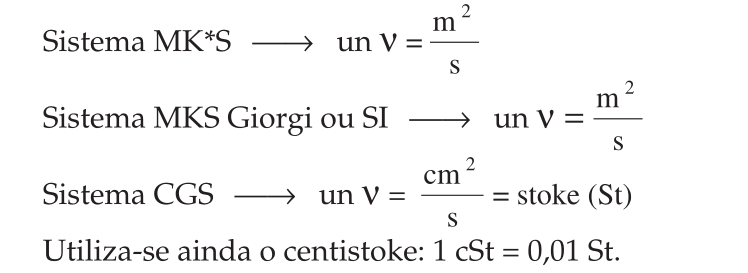
\includegraphics[width=\textwidth]{images/Captura de tela de 2025-03-26 16-54-30.png}
        \end{column}
    \end{columns}
\end{frame}
\begin{frame}{Exercícios do Livro Mecânica dos Fluidos de Franco Brunneti}
    \centering
    \includegraphics<+>[width=\textwidth]{images/Captura de tela de 2025-03-26 16-46-29.png}

    \includegraphics<+>[width=\textwidth]{images/Captura de tela de 2025-03-26 16-48-04.png}

    \includegraphics<+>[width=\textwidth]{images/Captura de tela de 2025-03-26 16-48-17.png}

    \includegraphics<+>[width=\textwidth]{images/Captura de tela de 2025-03-26 17-03-32.png}

    \only<.>{\vboxcorr{15pt}{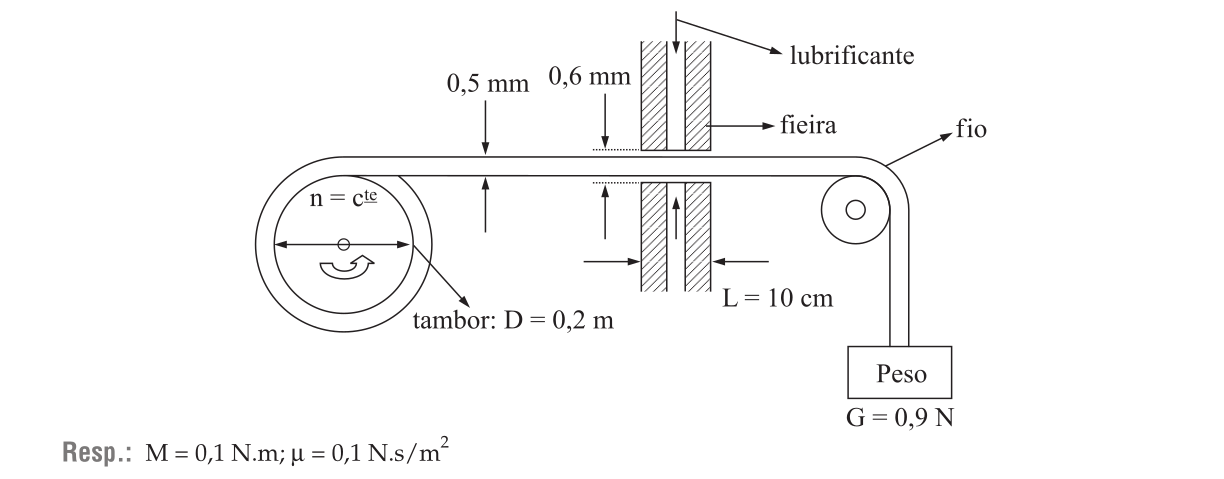
\includegraphics[width=\textwidth]{images/Captura de tela de 2025-03-26 17-03-50.png}}}

    \includegraphics<+>[width=\textwidth]{images/Captura de tela de 2025-03-26 16-37-14.png}

    \only<+>{\vboxcorr{23pt}{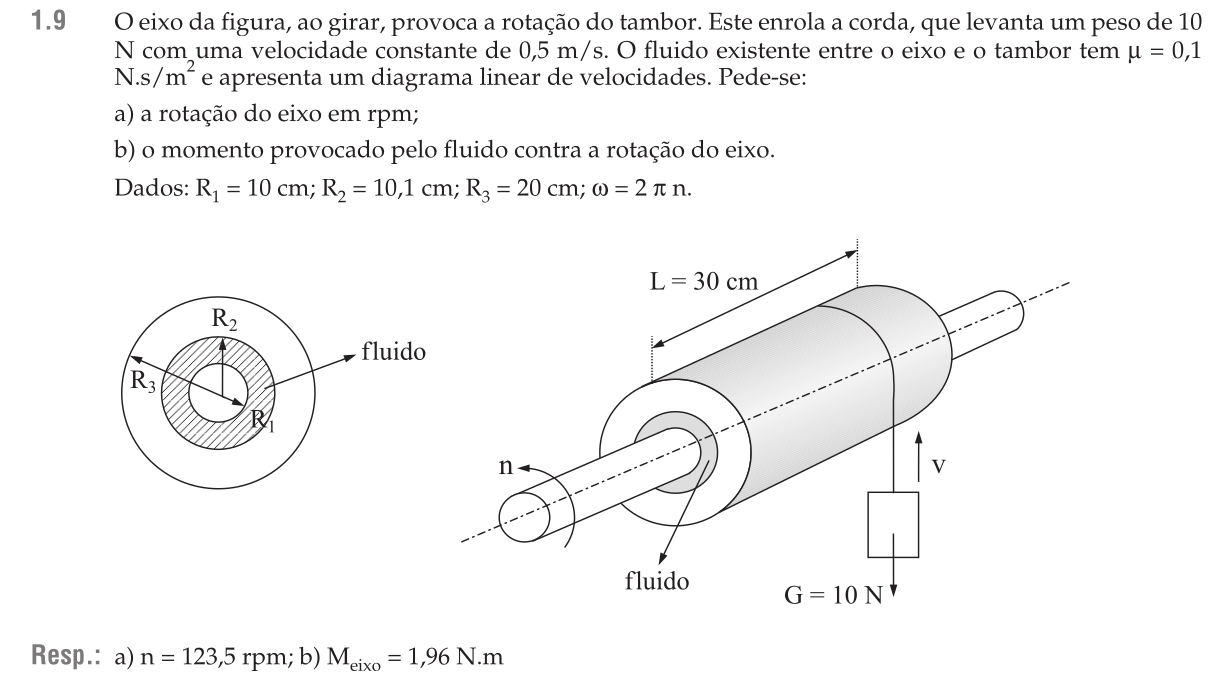
\includegraphics[width=\textwidth]{images/Captura de tela de 2025-03-26 17-07-59.png}}}

    \only<+>{\vboxcorr{2pt}{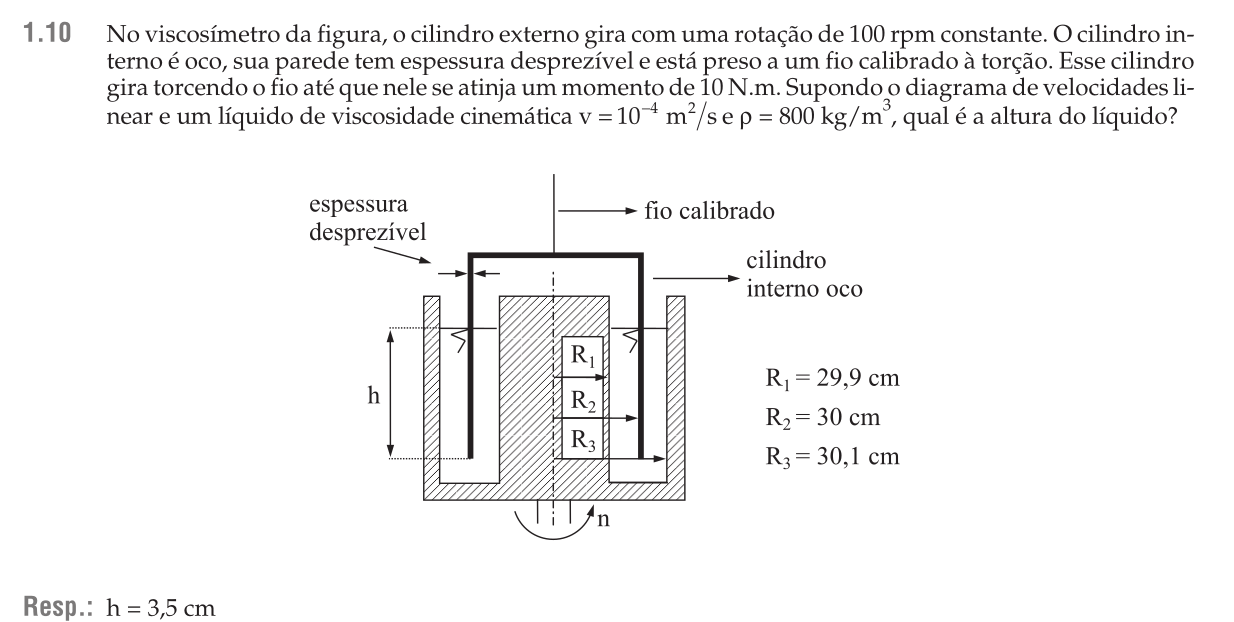
\includegraphics[width=\textwidth]{images/Captura de tela de 2025-03-26 17-22-38.png}}}

\end{frame}

 \begin{frame}{Revisão de Física Geral II}
     \centering 
     \includegraphics<+>[height=\textheight-28pt]{images/Captura de tela de 2025-04-01 15-36-19.png}

     \includegraphics<+>[height=\textheight-28pt]{images/Captura de tela de 2025-04-01 16-47-54.png}

     \includegraphics<+>[height=\textheight-28pt]{images/Captura de tela de 2025-04-01 15-37-11.png}

     \includegraphics<+>[height=\textheight-28pt]{images/Captura de tela de 2025-04-01 15-37-52.png}

 \end{frame}

 \begin{frame}{Revisão de Física Geral II}
     \begin{columns}[T]
         \begin{column}{0.45\textwidth}
             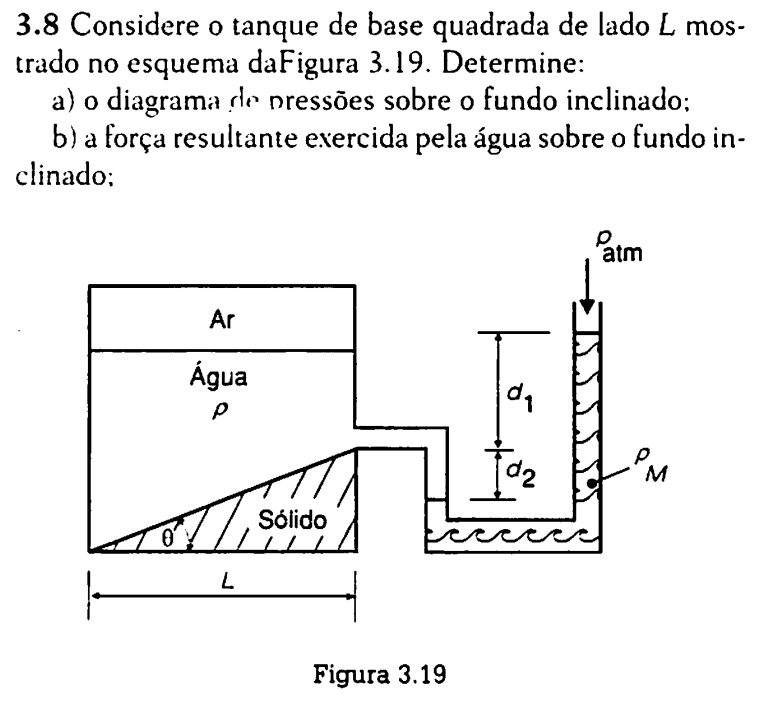
\includegraphics[width=\textwidth]{images/Captura de tela de 2025-04-01 15-55-30.png}
         \end{column}
%%%%%%%%%%%%%%%%%%%%%%%%%%%%%%%%%%%%%%%%%%%%%%%%%%
         \begin{column}{0.45\textwidth}

             \begin{tikzpicture}
                 \node [inner sep=0] (A) {
                     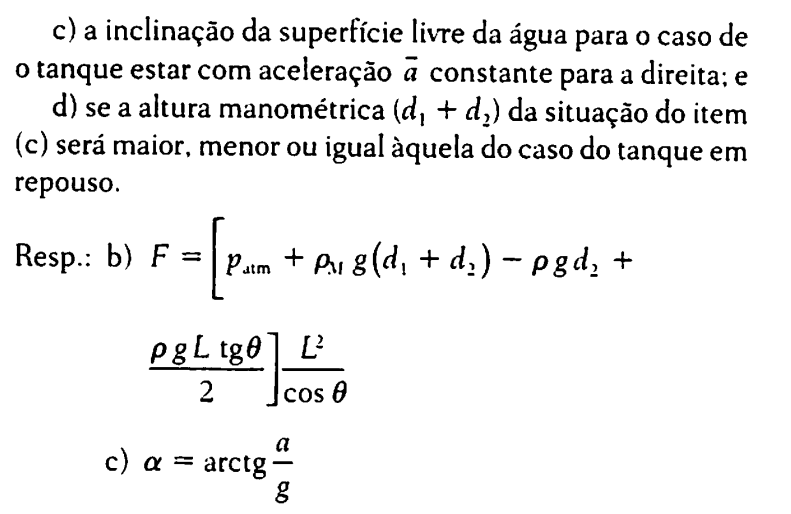
\includegraphics[width=\textwidth]{images/Captura de tela de 2025-04-01 15-55-44.png}
                 };


                 \coordinate (X0) at ($(A.south west)!0.00!(A.south east)$);
                 \coordinate (X1) at ($(A.south west)!0.99!(A.south east)$);
                 \coordinate (Y0) at ($(A.north west)!0.02!(A.south west)$);
                 \coordinate (Y1) at ($(A.north west)!0.40!(A.south west)$);
                 \filldraw [red, opacity=0.1] (X0|-Y0) rectangle (X1|-Y1);
             \end{tikzpicture}
         \end{column}
     \end{columns}
 \end{frame}


 \begin{frame}{Revisão de Física Geral II}
     \begin{columns}[T]
         \begin{column}{0.5\textwidth}
             \vboxcorr{44pt}{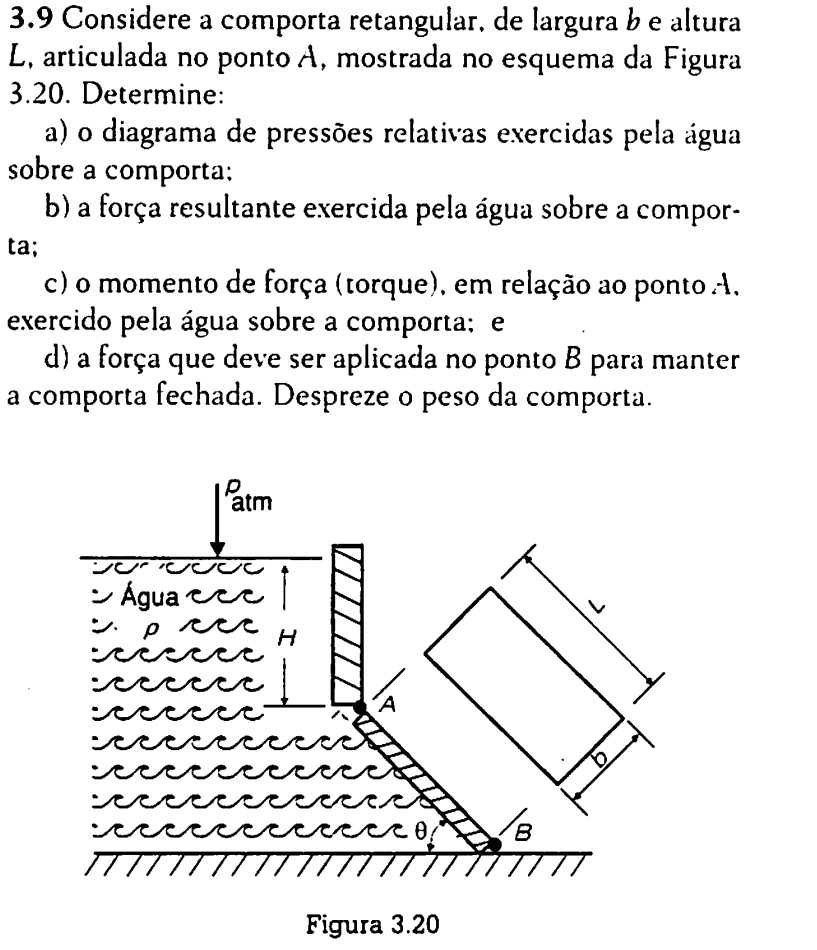
\includegraphics[width=\textwidth]{images/Captura de tela de 2025-04-01 17-06-56.png}}
         \end{column}

         \begin{column}{0.4\textwidth}
             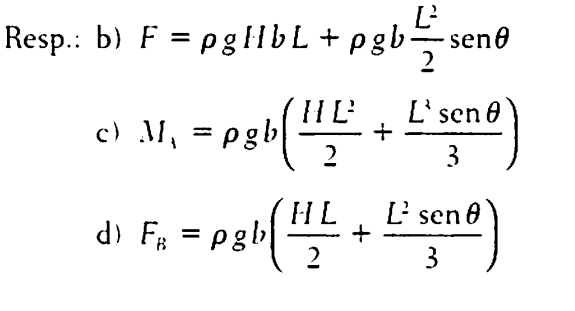
\includegraphics[width=\textwidth]{images/Captura de tela de 2025-04-02 16-47-44.png}
         \end{column}
     \end{columns}
 \end{frame}

 \begin{frame}{Revisão de Física Geral II}
     \centering
     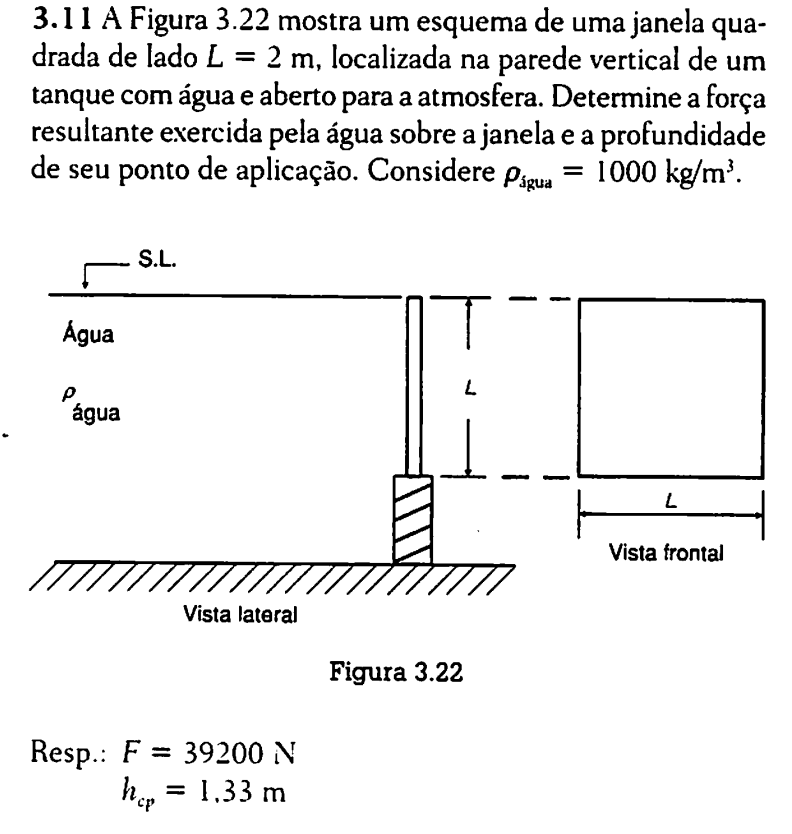
\includegraphics[height=\textheight-28pt]{images/Captura de tela de 2025-04-02 16-54-56.png}
 \end{frame}

 \begin{frame}{Revisão de Física Geral II}
     \begin{columns}[T]
         \begin{column}{0.5\textwidth}
             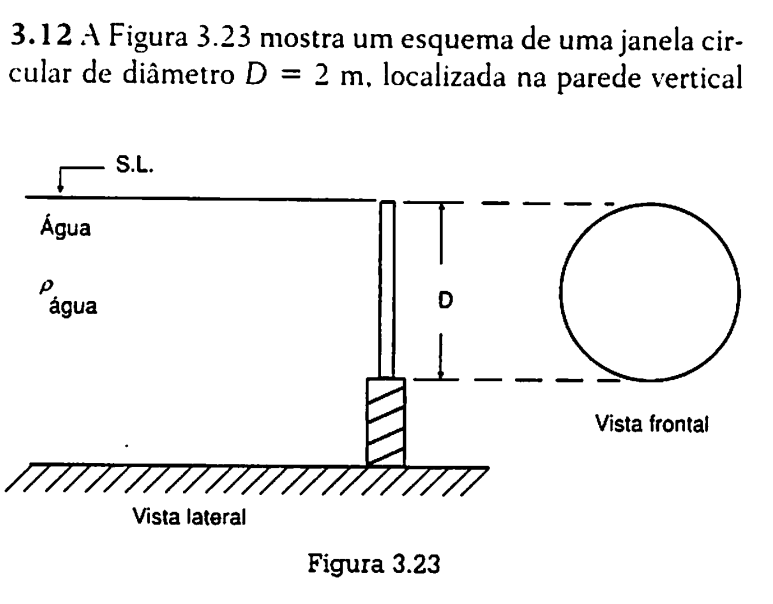
\includegraphics[width=\textwidth]{images/Captura de tela de 2025-04-02 16-55-06.png}
         \end{column}

         \begin{column}{0.4\textwidth}
             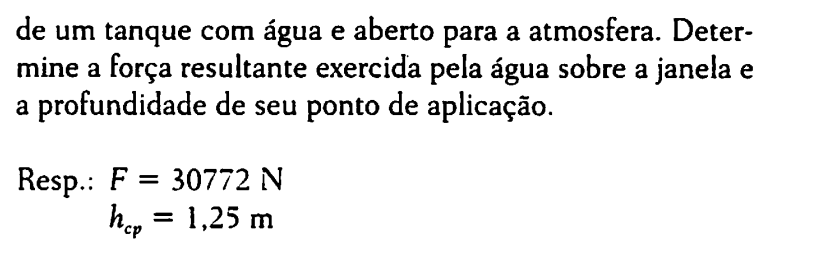
\includegraphics[width=\textwidth]{images/Captura de tela de 2025-04-02 16-55-20.png}
         \end{column}
     \end{columns}
 \end{frame}

\end{document}
